\section{Estado da Arte}
\label{cap:estado da arte}

Atualmente o uso de redes de computadores tem aumentado exponencialmente. Muitas dessas redes são distribuídas de forma geograficamente separadas precisando de uma complexa infra-estrutura de software e hardware para gerenciá-las e conectá-las. Dentre as diversas soluções existentes a grade computacional (\emph{grid computing}) possui característica que viabiliza essa conexão.

O Open Grid Forum (OGF) uma comunidade fórum com milhares de indivíduos representando mais de 400 organizações em mais de 50 países criou e documentou \cite{M.2002} especificações técnicas e experiências de usuários. O OGF definiu grades computacionais como um ambiente persistente o qual habilita aplicações para integrar instrumentos, disponibilizar informações em locações difusas. Desde lá esta não é a única e precisa definição para o conceito de grades. Foster \cite{Kesselman2001} define um sistema em grade propondo um \emph{checklist} de três pontos.

\begin{enumerate}
	\item coordenar recursos os quais não são direcionados para um controle central.
	\item usar protocolos e interfaces padronizados, abertos para propósitos gerais.
	\item oferecer QoS (qualidade de serviço) não triviais tais como: autenticação, escalonamento de tarefas, disponibilidade.
\end{enumerate}

Uma definição formal do que um sistema em grade pode prover foi definido em \cite{Foster2002}. Focando na sua semântica, mostrando que grades não são apenas uma modificação de um sistema distribuído convencional. Podem apresentar recursos heterogênicos como sensores e detectores e não apenas nós computacionais. Abaixo uma lista de aspectos que evidenciam uma grade computacional \cite{Cirne2002}:

\begin{itemize}
	\item heterogeneidade
	\item alta dispersão geográfica
	\item compartilhamento ( não pode ser dedicado a uma única aplicação )
	\item múltiplos domínios administrativos ( recursos de várias instituições )
	\item controle distribuído 
\end{itemize}

A grade deve estar preparada para lidar com todo o dinamismo e variabilidade, procurando obter a melhor performance possível adaptando-se ao cenário no momento.

Devido à grande escala, ampla distribuição e existência de múltiplos domínios administrativos, a construção de um escalonador de recursos para grades é praticamente inviável, até porque, convencer os administradores dos recursos que compõem a grade abrirem mão do controle dos seus recursos não é uma tarefa nada fácil. Escalonadores têm como características receber solicitações de vários usuários, arbitrando, portanto, entre os usuários, o uso dos recursos controlados.  

Casavant \cite{Thomas1996} considera escalonar como um problema de gerenciamento de recursos. Basicamente um mecanismo ou uma política usada para, eficientemente e efetivamente, gerenciar o acesso e uso de um determinado recurso. Porém, de acordo com o OGF's \cite{M.2002}, escalonamento é o processo de ordenar tarefas sobre os recursos computacionais e ordenar a comunicação entre as tarefas, assim sendo, ambas aplicações e sistemas devem ser escalonadas. 

O gerenciamento de recursos de um sistema centralizado possui informação completa e atualizada do status dos recursos gerenciados. Este difere do sistema distribuído, o qual não tem conhecimento global de recursos dificultando assim, o gerenciamento. O ambiente em grade introduz cinco desafios para o problema de gerenciamento de recursos em ambientes distribuídos \cite{Karl1998}:

\begin{enumerate}
\item autonomia: os recursos são, tipicamente propriedades e operados por diferentes organizações em diferentes domínios administrativos.
\item heterogeneidade: diferentes lugares podem usar diferentes sistemas de gerenciamento de recursos (RMS - \emph{resource management system}).
\item extender as políticas: suporte no desenvolvimento de nova aplicação de mecanismos de gerência num domínio específico, sem necessitar de mudanças no código instalado nos domínios participantes.
\item co-alocação: algumas aplicações tem necessidades de recursos os quais só podem ser satisfeitos apenas usando recursos simultâneos com vários domínios.
\item controle online: RMSs precisam suportar negociações para adaptar necessidades de aplicações para recursos disponíveis.
\end{enumerate}

\subsection{Gerenciamento de Aplicações}

Sistemas computacionais, na sua grande parte, falham ao tratar dois problemas \cite{Mangan2006}: (1) gerenciamento e controle de um grande número de tarefas; (2) o balanceamento da carga da máquina de submissão e do tráfego da rede.

Uma distribuição dinâmica de dados e tarefas em uma hierarquia de gerenciadores poderia ajudar o gerenciamento de aplicações. Um modelo denominado GRAND (\emph{Grid Robust Application Deployment}) baseado na submissão e controle particionados e hierárquicos foi proposto em \cite{Mangan2006}

Pelo fato de que, na atualidade, ambientes grades envolvem principalmente instituições de ensino em aplicações usualmente classificadas como aplicações científicas, o escopo do GRAND é limitado as seguintes itens. 1- heterogeneidade, lembrando que isto afeta diretamente a política de escalonamento por necessitar de saber as características distintas de hardware e software; 2- grande número de submissão de tarefas, referindo-se a aplicações que geram centenas ou milhares de processos; 3- ausência de comunicação por troca de mensagens, pelo fato da necessidade de inúmeros aspectos nas fases de agrupamento e mapeamento serem considerados; 4- interdependência de tarefas, devido ao compartilhamento de arquivos; 5- manipulação de grande número de arquivos pelas tarefas; 6- o uso de arquivos grandes, através técnicas como \emph{staging} e \emph{caching}, minimizando a perda de desempenho em função da latência de transmissão; 7- segurança, assume-se que exista uma conexão segura entre os nós da grade; 8- descoberta dinâmica de recursos; 9- gerenciador de recursos local em cada nó; 10- uma tarefa é executada em um RMS até sua finalização;

No modelo GRAND são tratados três aspectos do gerenciamento de dados: transferência automática dos dados de entrada para o local onde o arquivo será necessário; o envio de resultados é controlado evitando congestionamento da rede; priorização de localidade no disparo de tarefas para não haver transferências desnecessárias de dados degradando o desempenho. Através de uma hierarquia de gerenciadores (figura 1) é feito o disparo e controle das aplicações. o \emph{Application Manager} (AP) recebe uma submissão de aplicação através de um usuário, os APs mandam os \emph{Submission Manager} (SM) descrições de tarefas assim, sob demanda, são instanciados os \emph{Task Managers} (TM) para controlar a submissão de tarefas a escalonadores de domínios específicos da grade, esses escalonadores recebem requisições dos TMs fazendo a execução das tarefas propriamente ditas.

\begin{figure}[h]
\center
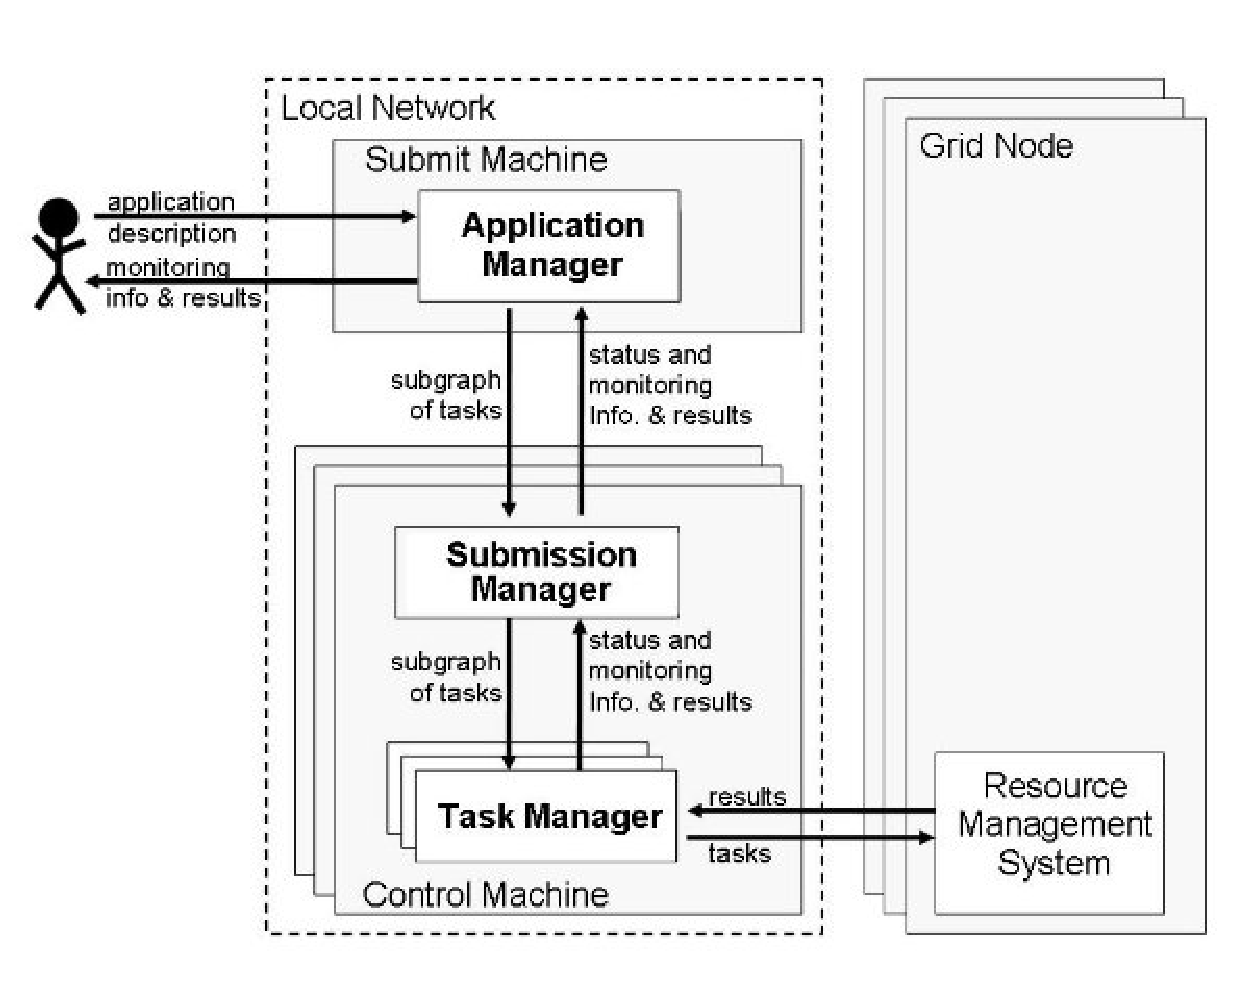
\includegraphics[scale=.6]{img/grand.eps}
\label{grand}
\caption{Principais componentes do modelo hierárquico de gerenciamento de tarefas}
\end{figure}

O AppMan usa o serviço provido pelo EXEHDA middleware \cite{Nino2006} que libera monitoramento e execução remota. As características básicas do GRAND foram implementadas no AppMan, inclusive a submissão de tarefas e o retorno para o usuário. Em cada nó da grade é necessário estar sendo executada uma instância do ISAM/EXEHDA e do AppMan. Qualquer máquina pode submeter ou executar tarefas. A tarefa do AppMan é garantir o escalonamento das tarefas assim como a autorização e autenticação das tarefas executadas. Ele consiste num gerenciador que dispara e controla cada aplicação nos nós com base nas informações recebidas do pelo gerenciador de submissão. O gerenciador de submissão, além de enviar informações, cria e monitora os gerenciadores de tarefas. Os gerenciadores de tarefas são responsáveis pela comunicação com o escalonador de um determinado domínio garantindo a execução remota e a ordem das tarefas de acordo com a dependência de dados \cite{Mangan2006}.
